\section{MC simulations}
\label{sec:sim}
\subsection{The Hall-A high-power beam-dump}
The Hall A and C use identical high-power absorbing (up to 1 MW)  beam-dumps to stop the 11 GeV beam, remnant of beam/target interaction. The dump is made by a set of about 80 aluminum disks, each
approximately 40 cm in diameter of increasing thickness (from 1 to 2 cm), for a total
length of approximately 200 cm, followed by a solid Al cylinder 50cm in diameter
and approximately 100 cm long. They are both cooled by circulating water. The full
drawing of the beam-dump is shown in Fig.~\ref{fig:bd}. To increase the radiation shielding,
the thickness of the concrete tunnel surrounding the Al dump is about 4-5 m thick.

\begin{figure}[h!] 
\center
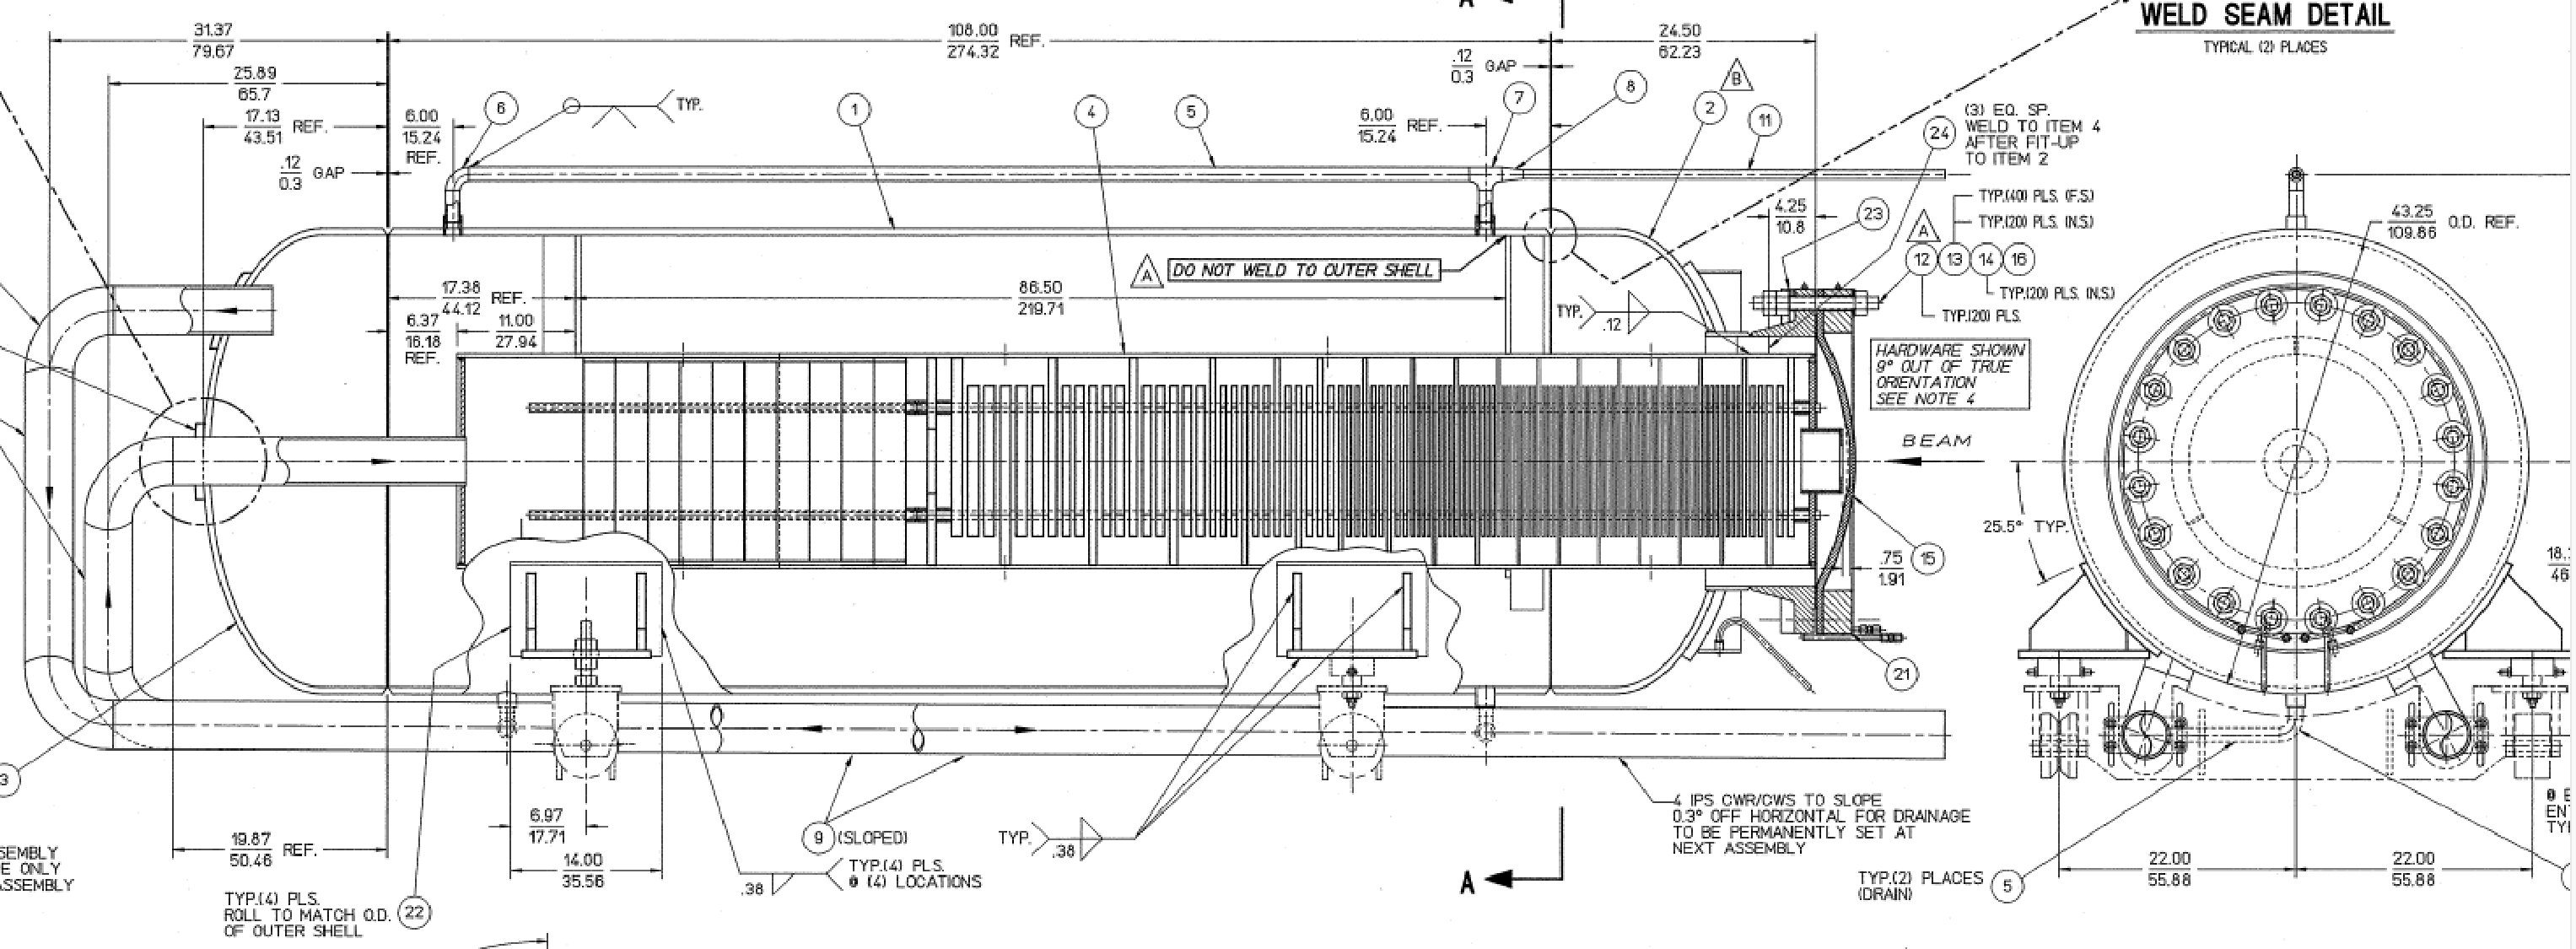
\includegraphics[width=7.5cm]{figs/beam-dump-br.pdf}
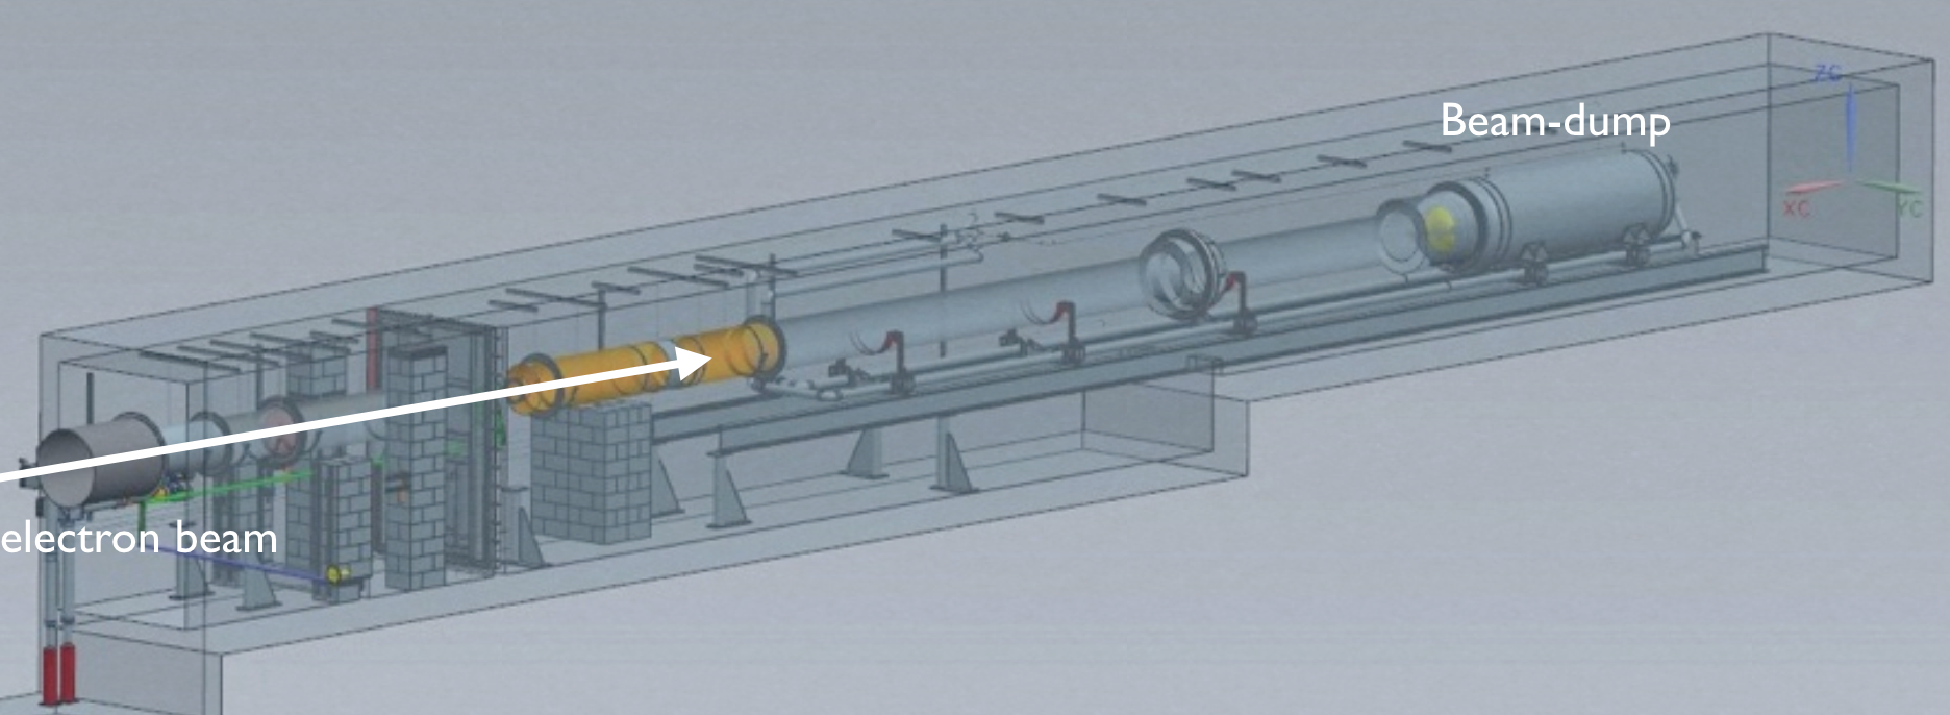
\includegraphics[width=7.5cm]{figs/beam-dump.pdf}
\caption{Hall-A beam dump and beam dump enclosure. }
\label{fig:bd}
\end{figure}

\subsection{The beam-dump model in FLUKA}
The beam-dump geometry and  materials have  been implemented in FLUKA-2011.2c.5 by the Jefferson Lab Radiation Control Department. Detailed are reported in Ref.~\cite{jnote-bd}.  The input card used to run the program  includes all physics process and a tuned set of bias to speed up the running time not affecting the results integrity. 
\begin{figure}[h!] 
\center
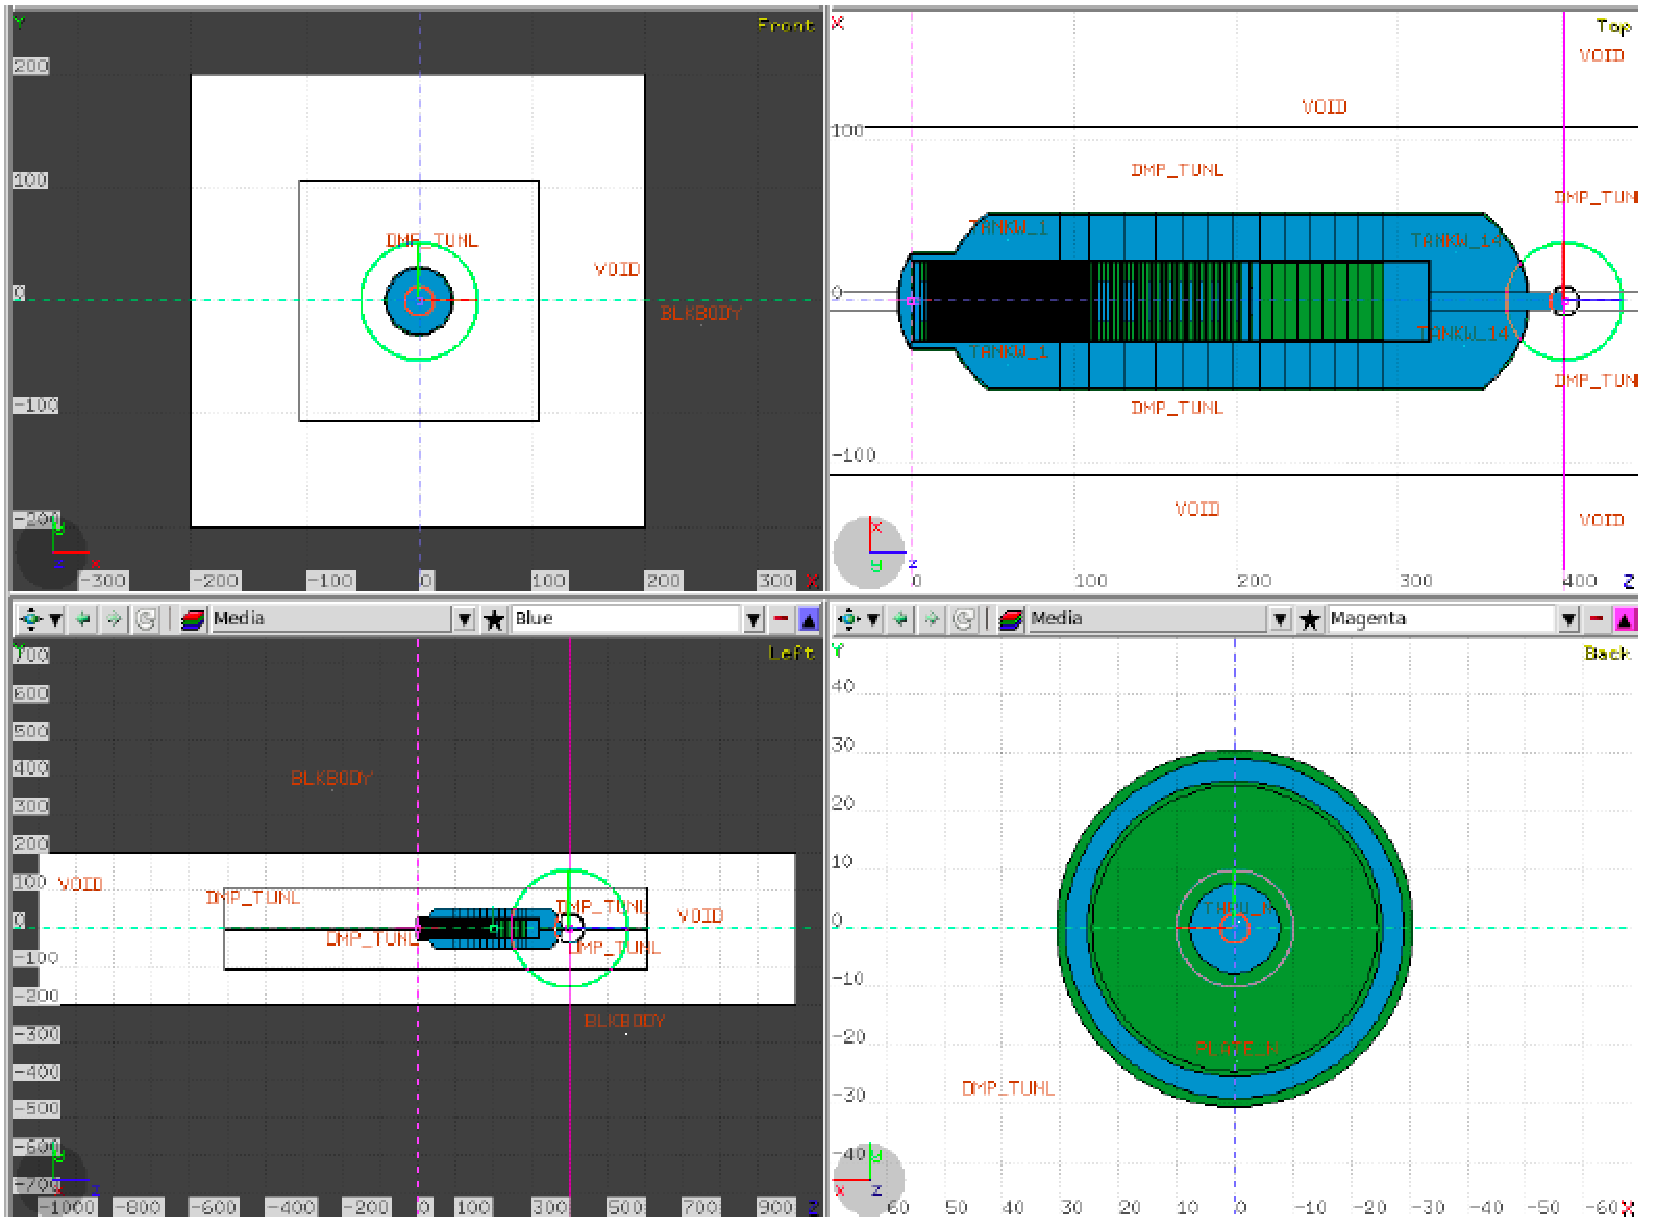
\includegraphics[width=12.5cm]{figs/fluka-bd.pdf}
\caption{Hall-A beam-dump implementation in FLUKA. }
\label{fig:fluka-bd}
\end{figure}
The $\mu$, n, and $\gamma$ fluence (differential in angle and energy) per EOT were  calculated   at XXX cm  downstream of the beam window, through a circular area of 105 cm$^2$. Figure~\ref{fig:fluka-bd} shows the FLUKA graphic representation and the location of the flux detector.
An extension to also include the proper geometry and material composition downstream of the beam-dump has also been implemented.
Figure~\ref{fluka-bd-dwns}  shows the geometry of of the concrete bunker surrounding the beam-dump and  the soil as implemented in FLUKA.

\begin{figure}[h!] 
\center
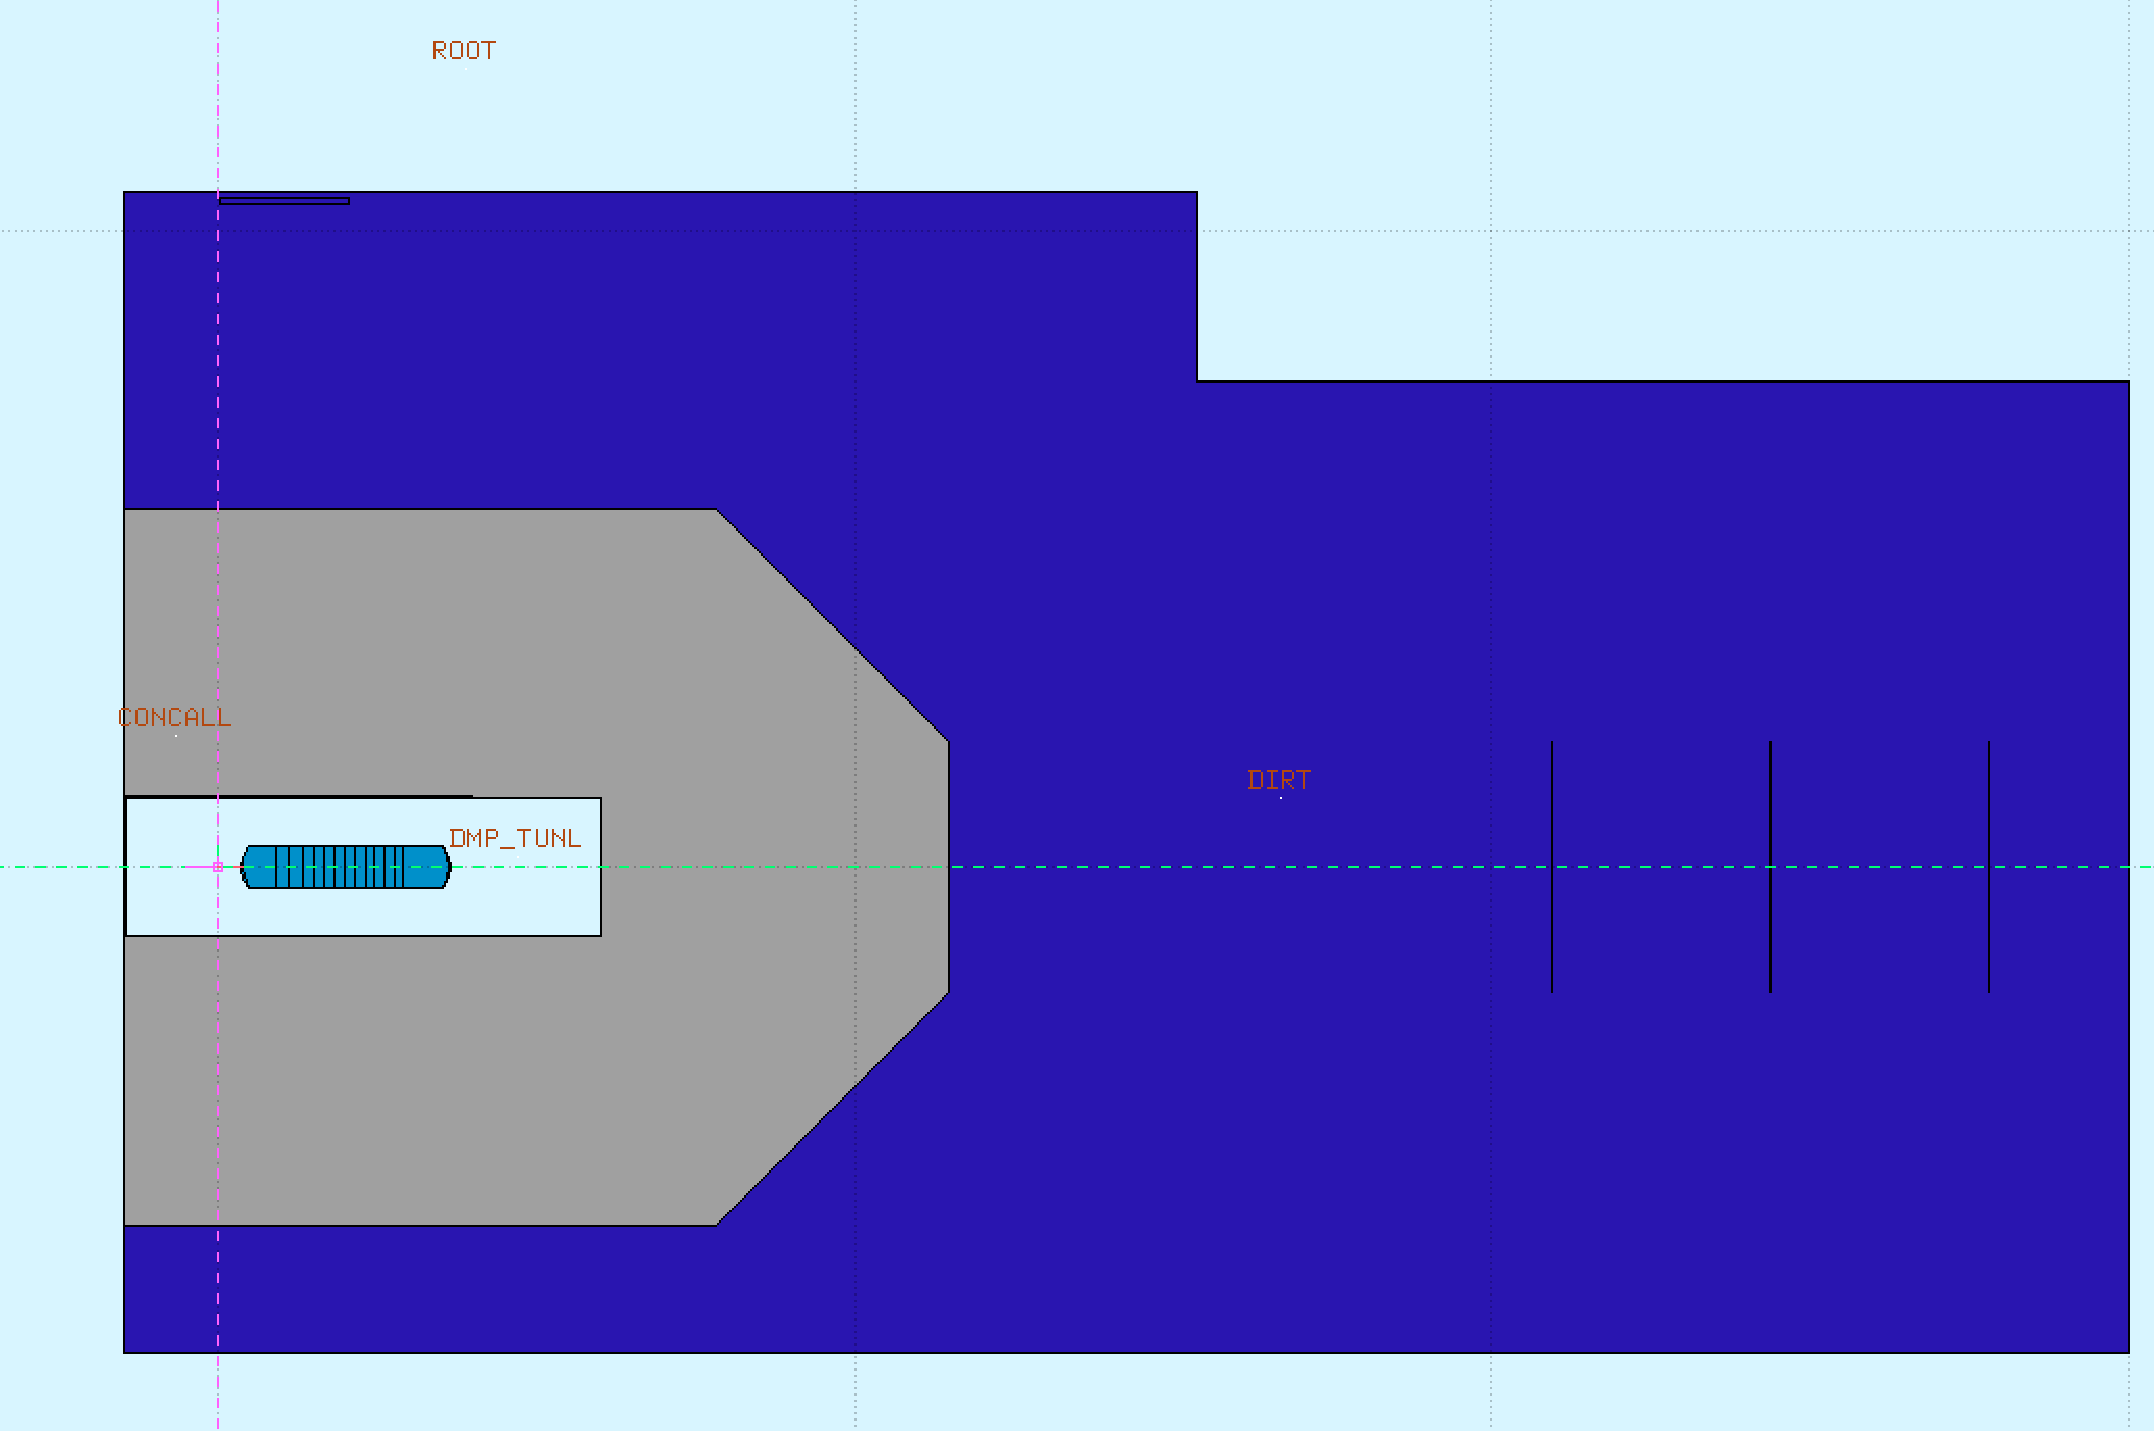
\includegraphics[width=12.5cm]{figs/fluka-bd-dwns.pdf}
\caption{The geometry/composition  of the concrete bunker surrounding the beam-dump and  the soil as implemented in FLUKA.}
\label{fig:fluka-bd-dwns}
\end{figure}


\subsection{The beam-dump model in GEANT4 (GEMC)}
The beam-dump model, as well as the geometry and composition  of surrounding proximity,
 has also been implemented in GEANT4 using the GEMC tool~\cite{gemc}. This is a refined version with-respect-to the one used  in PR-16-001~\cite{bdx-proposal} that better matches the beam-dump geometry implemented in FLUKA. For a better description of  muon transportation, the {\tt G4GammaConversionToMuons} has been added to the standard physics list used in simulations of  PR-16-001({\tt FTFP\_BERT\_HP + STD + HP}).
Particles flunce has been sampled  by mean of a  a flux detector has been positioned in the same location as in the FLUKA model.
Figure~\ref{ig:gemc-bd-dwns} shows the beam dump and vicinity implemented in GEMC.
\begin{figure}[h!] 
\center
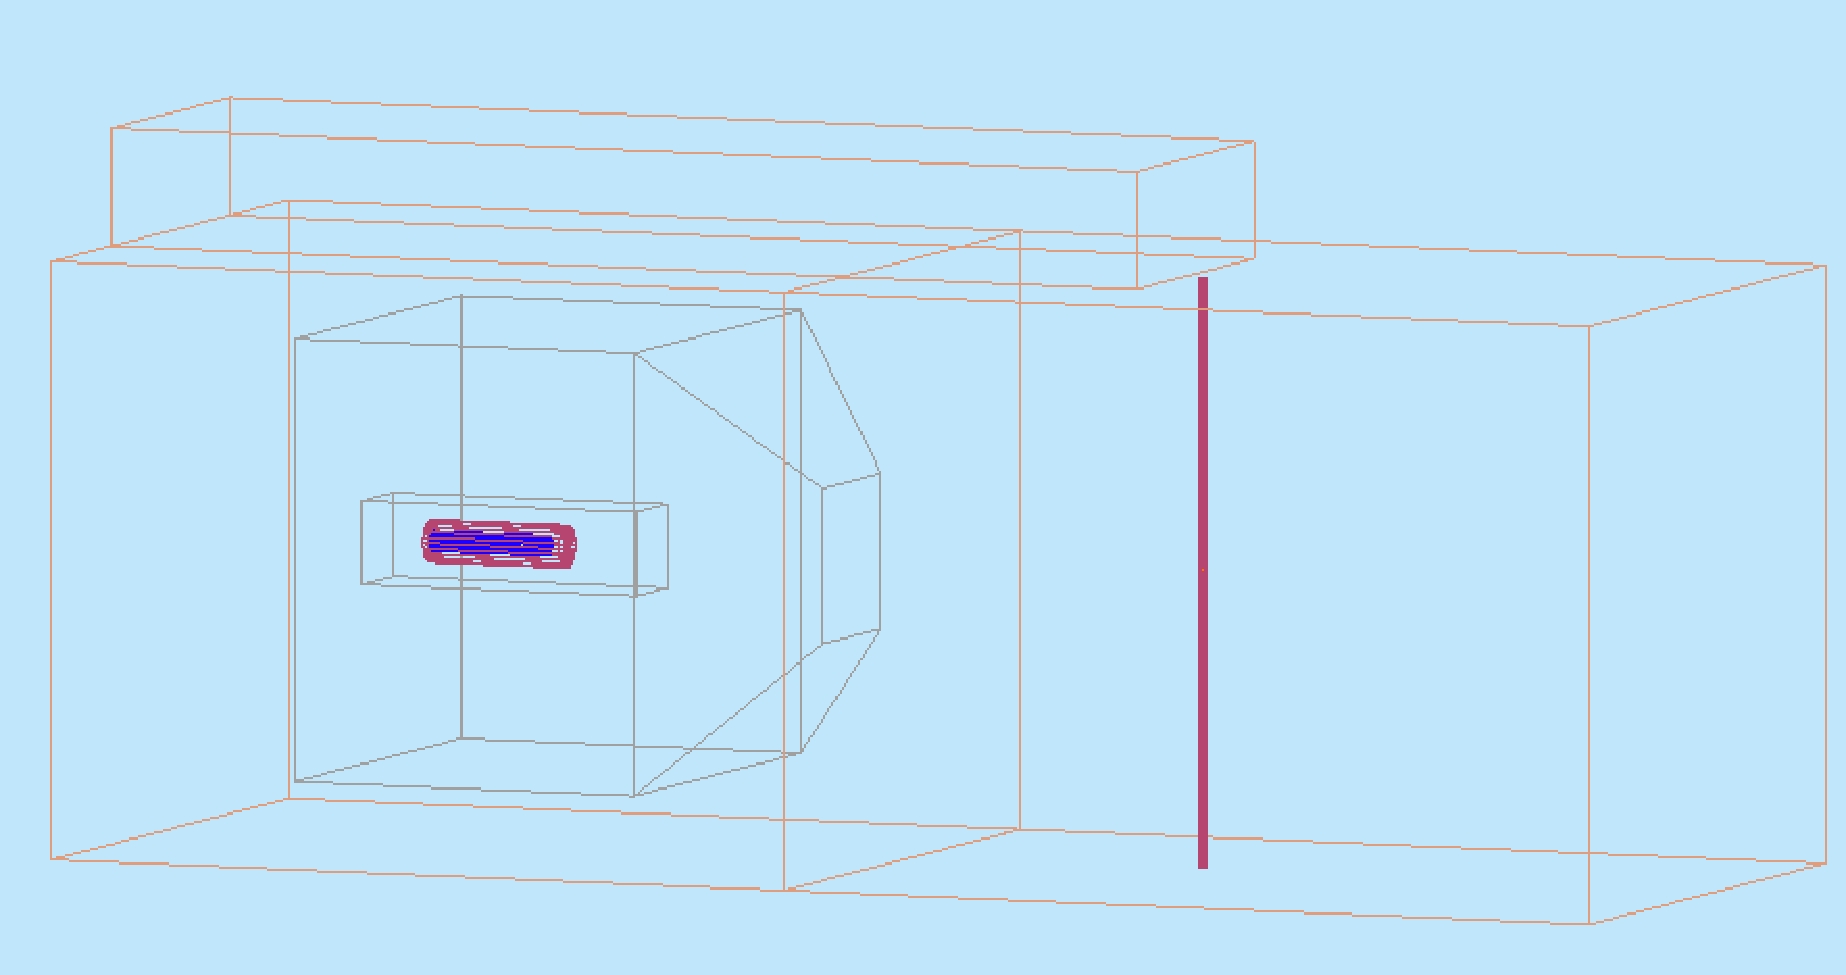
\includegraphics[width=12.5cm]{figs/gemc-bd-dwns.pdf}  
\caption{The geometry/composition  of the beam-dump, the sourraunding concrete bunker and  the soil as implemented in GEMC.}
\label{fig:gemc-bd-dwns}
\end{figure}
\subsection{Muons from beam/dump interaction}
A comparison of muon fluence downstream of the beam-dump (see above for details about the location)
obtained by FLUKA and GEMC are reported in Fig.~\ref{mu-flu-bd}. Considering that low energy muons are absorbed by the bunker-head shielding, to keep the GEMC running time reasonable, only particles (all) with energy grater than 100 MeV ({\tt ENERGY\_CUT=100*MeV}) has been tracked and sampled. A total of 4$\times10^9$ ($9\times 10^6$) EOT have been simulated with GEMC (FLUKA). The comparison of the two simulations shows a perfect agreement in the full energy range where data were generated.
In spite of a factor of $\times$100  less statistics, FLUKA shows, as expected, smaller error bars. This reflects the optimised sizes used by the simulation to generate high statistics for low probability processes keeping the total statistics limited.
To penetrate  the concrete shielding and the soil,  minimum energy of  E$_\mu>4$ GeV is required. With this energy cut,   the integrated number of muon per EOT results in $4.8\pm 0.1 \times 10^{-7}$ ($5.5\pm 0.2 \times 10^{-7}$) for GEMC and FLUKA respectively.
Figure~\ref{mu-flu-bd-2d} show the correlation between the muon energy and the azimuthal angle (with-respect-to the beam-line): the regions that are populated by both simulations, show again, the same behaviour.

\begin{figure}[h!] 
\center
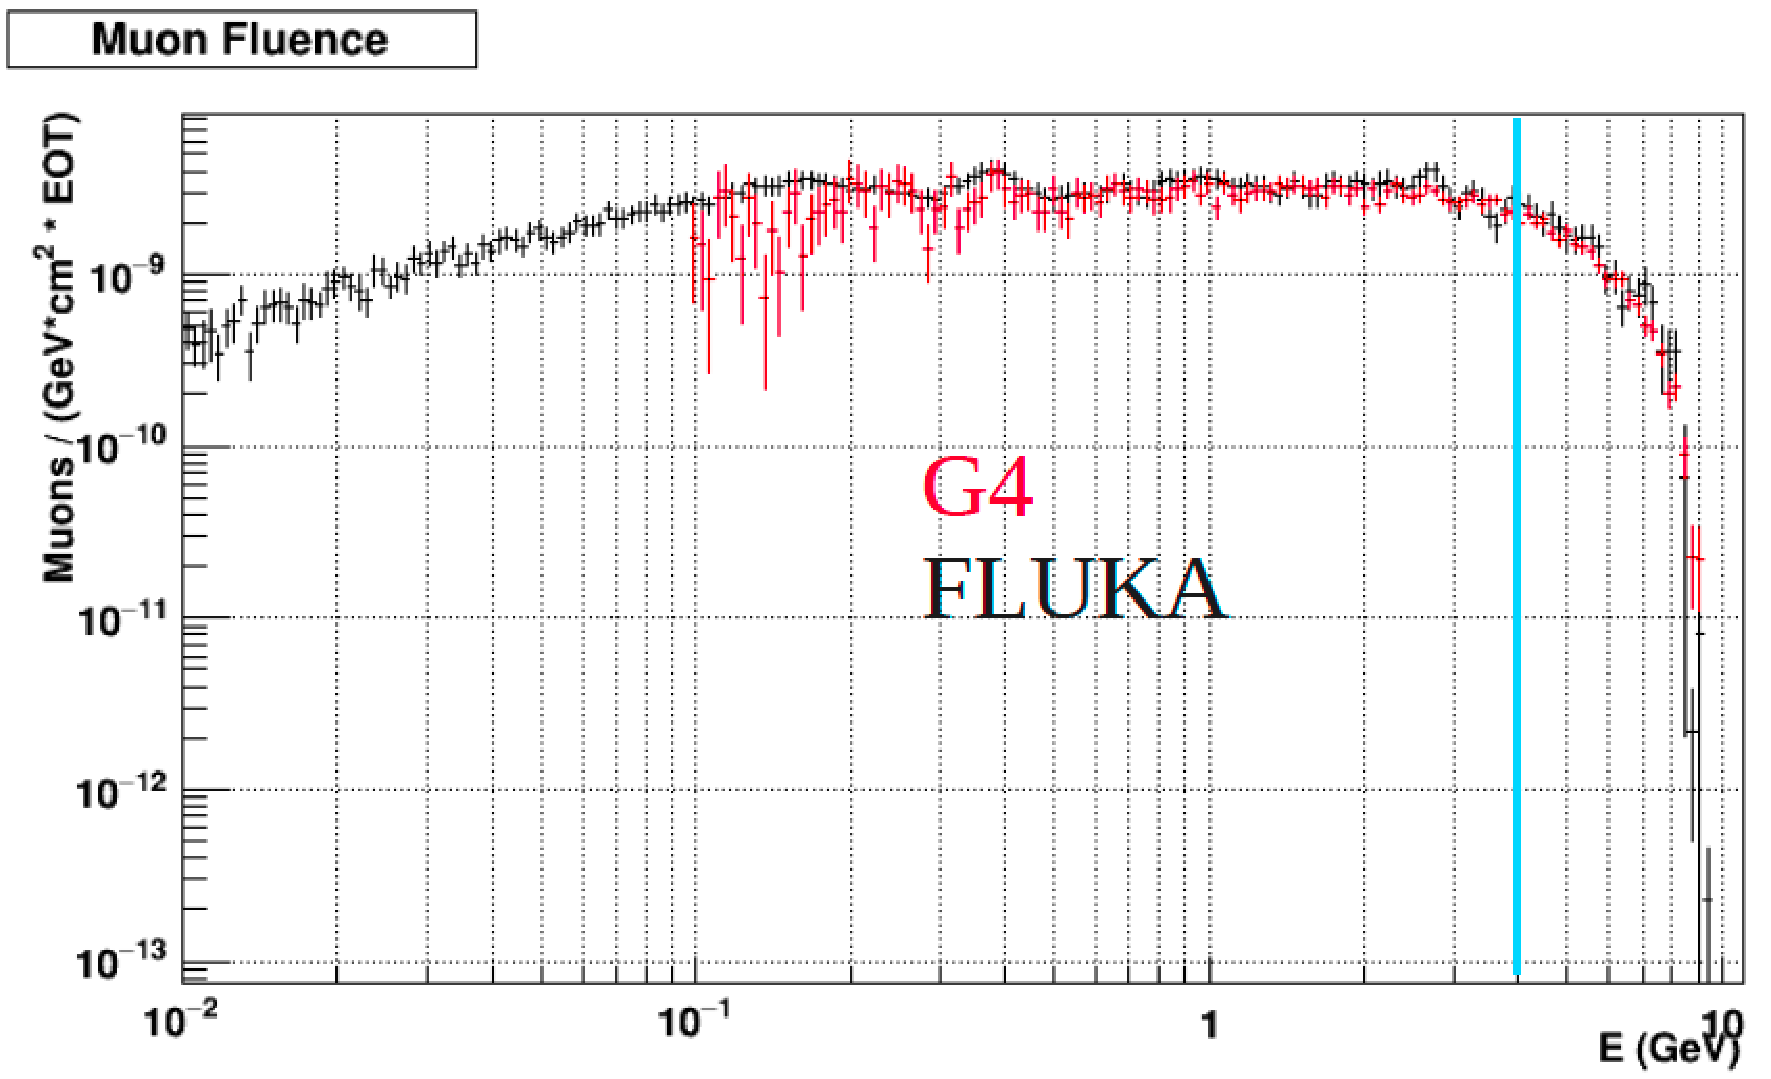
\includegraphics[width=8.5cm]{figs/mu-flu-bd.pdf}
\caption{Muon fluence downstream of the beam-dump obtained by FLUKA (black) and GEMC (red). The GEMC simulations started at E$\mu=$100 MeV.}
\label{fig:mu-flu-bd}
\end{figure}

\begin{figure}[h!] 
\center
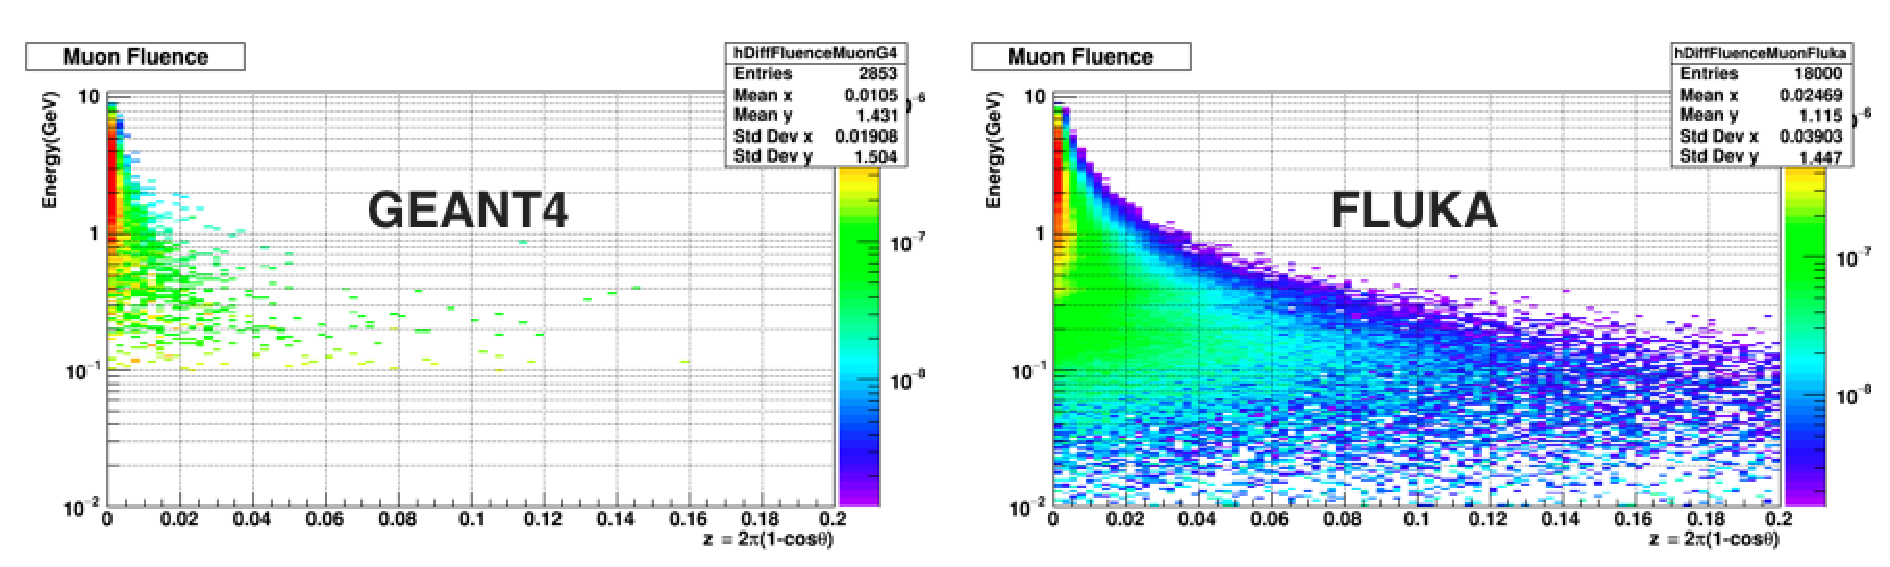
\includegraphics[width=16cm]{figs/mu-flu-bd-2d.pdf} 
\caption{Energy vs. azimuthal angle of muons crossing the flux detector located downstream of the beam-dump obtained by FLUKA  and GEMC.}
\label{fig:mu-flu-bd-2d}
\end{figure}


\subsection{Sampling  and particle transport}\label{sec:sampling}
The good agreement between two independent simulation tools (FLUKA and GEMC)  gives us confidence about reliability of the obtained results. Both methods have pros and cons. FLUKA shows a superior speed in running but a complicated implementation and of selected results (e.g. the final output is given via {\it scores} such as fluence or distribution in specific location  need to be pre-defined ). GEMC (GEANT4) tracks particles in all volumes providing a straightforward  output (particle four-momenta) in the desired flux detector but requires an un-practical running time to collect a reasonable statistics (in particular when an em shower is involved). In the following we describe how we overtook these difficulties.

\subsubsection{Muons - GEMC}\label{sec:gmc-mu}
We used GEMC to simulate muons. To make the  process more efficient, we followed the   procedure described below: 
\begin{itemize}
\item  we used a low statistic sample of EOT to simulate the interaction of the 11 GeV electrons with the beam-dump;
\item  we sampled the muon flux and variables (momentum, azimuthal angle and transverse position)  on a flux detector located downstream of the beam-dump;
\item we use the distributions from previous step as input of a custom event-generator to produce a high statistic muon sample;
\item we used GEMC to transport muons  downstream of the beam dump all the way up the desired location of the BDX-Hodo;
\item  we implemented  the  BDX-Hodo response in GEMC to realistically describe the muon detection.
\end{itemize}
The position where muons are sampled from the primary beam/dump interaction and generated in the custom-made event generator is shown in Fig.~\ref{fig:mu-gen}.

\begin{figure}[h!] 
\center
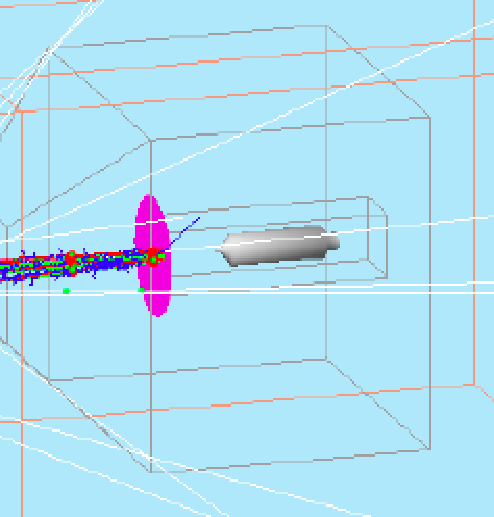
\includegraphics[width=12cm]{figs/mu-gen.pdf}   
\caption{The position of $\mu$ sampling/generation.}
\label{fig:mu-gen}
\end{figure}


Figure~\ref{fig:mu-sampling} shows the muon distributions (energy vs azimuthal angle and radial distance from the beam line ) downstream of the beam-dump, as obtained by the full GEMC simulation of  11 GeV electrons hitting the beam-dump.
The left panel of Fig.~\ref{fig:mu-sampling-extract} shows the comparison one of the two distributions as obtained by the GEMC with the result of the custom event generator. 
As a check, the right panel of the same figure  shows the same comparison in the location of interest, $\sim 20$ m downstream of the beam-dump.
The difference in the error bar size indicates the improvement obtained by this procedure with-respect-to  the limited statistic from GEMC. 

\begin{figure}[h!] 
\center
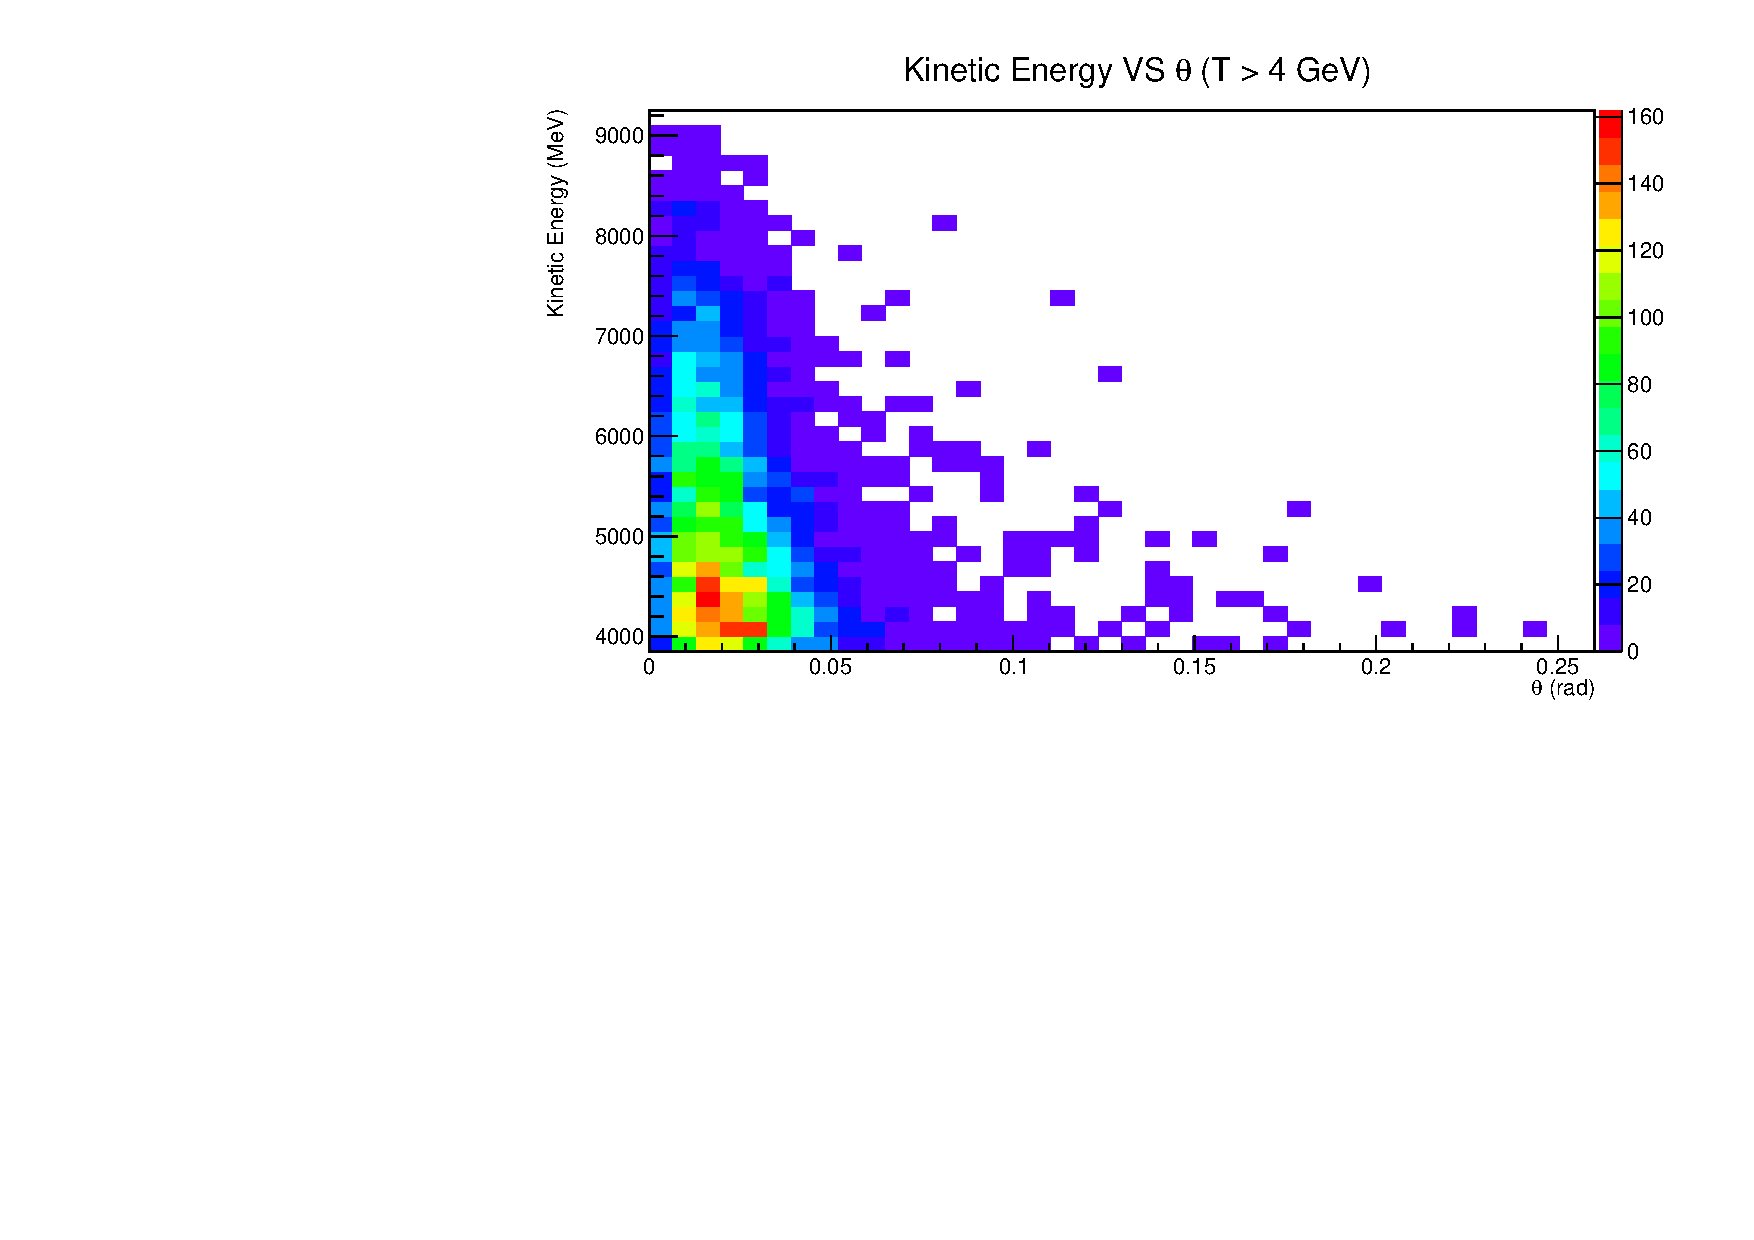
\includegraphics[width=7.5cm]{figs/EkinVStheta.pdf}
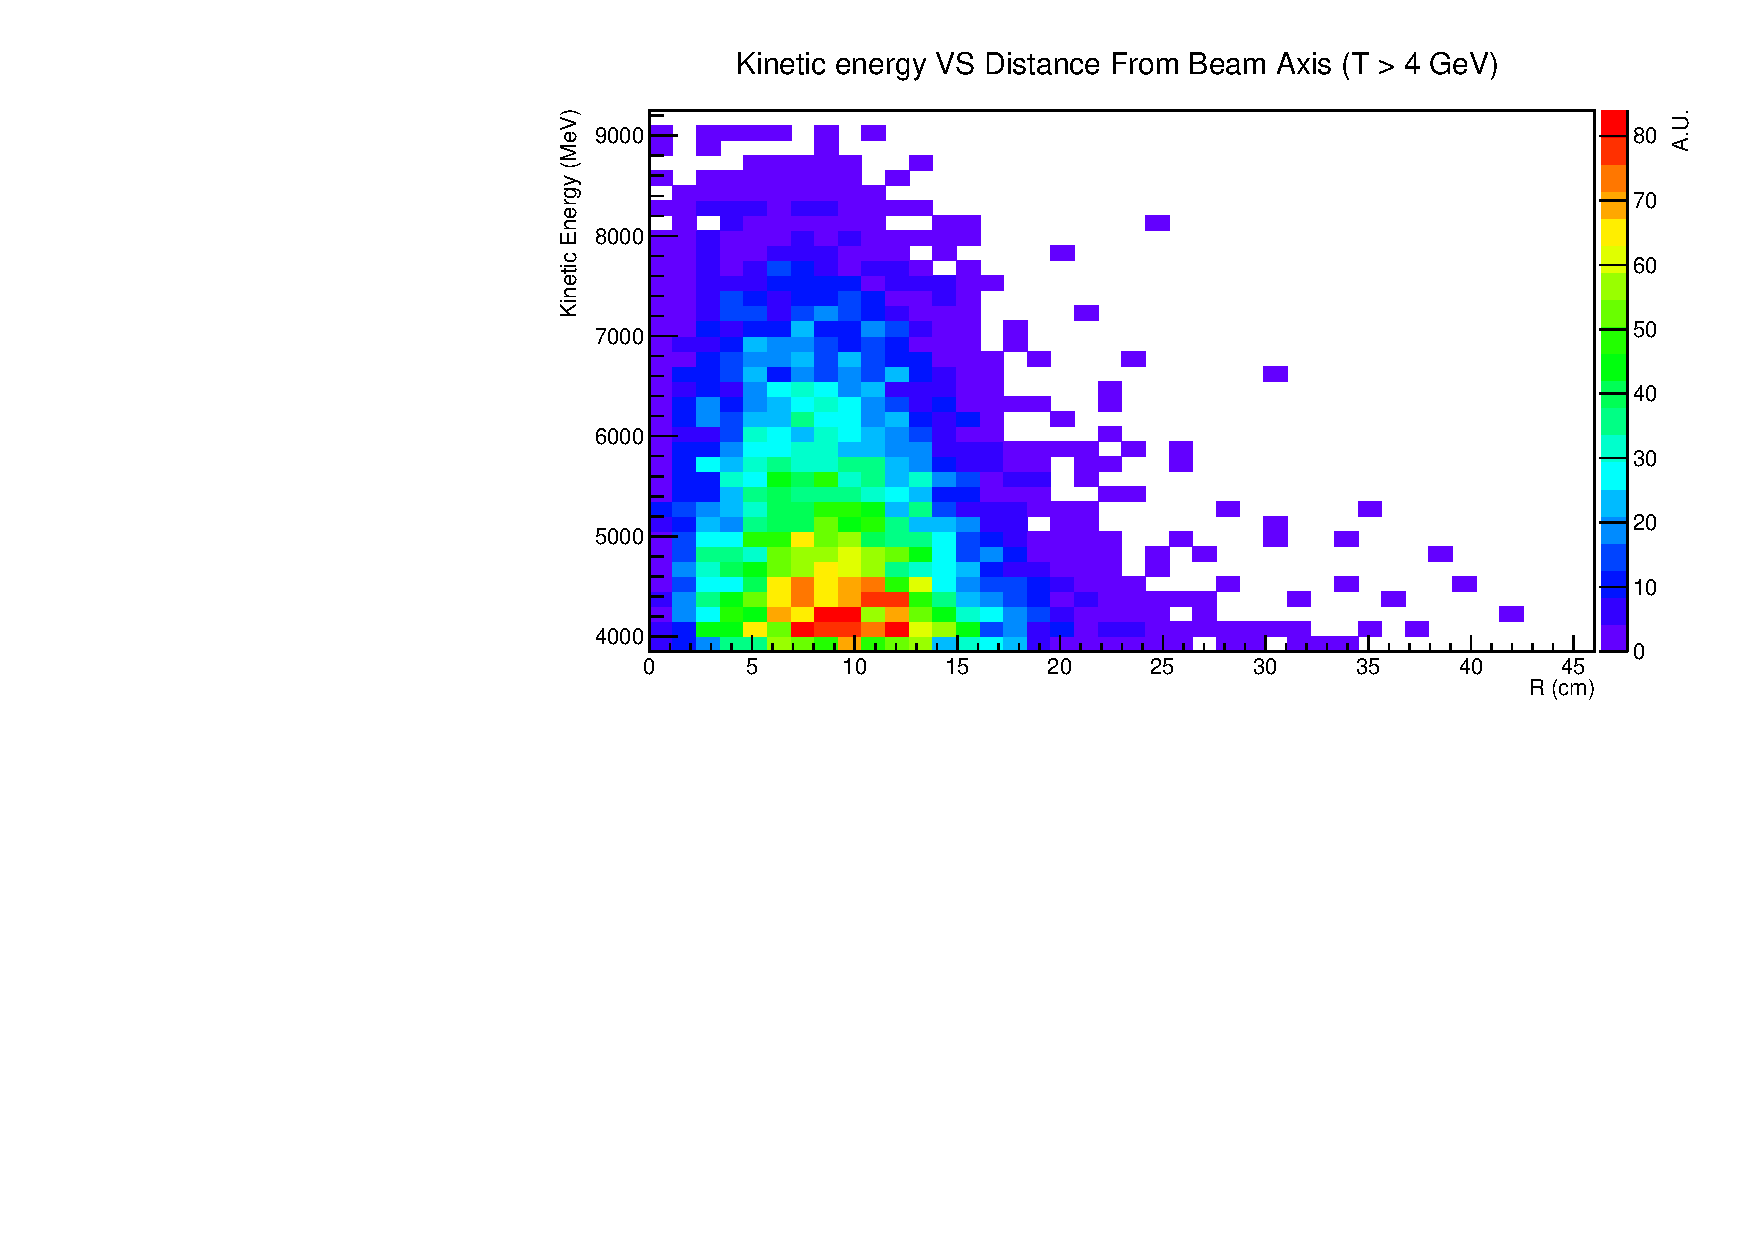
\includegraphics[width=7.5cm]{figs/EkinVSR.pdf}
\caption{Muon kinetic energy vs. azimuthal angle (left) and distance (right) from the beam-line axes.}
\label{fig:mu-sampling}
\end{figure}
\begin{figure}[h!] 
\center
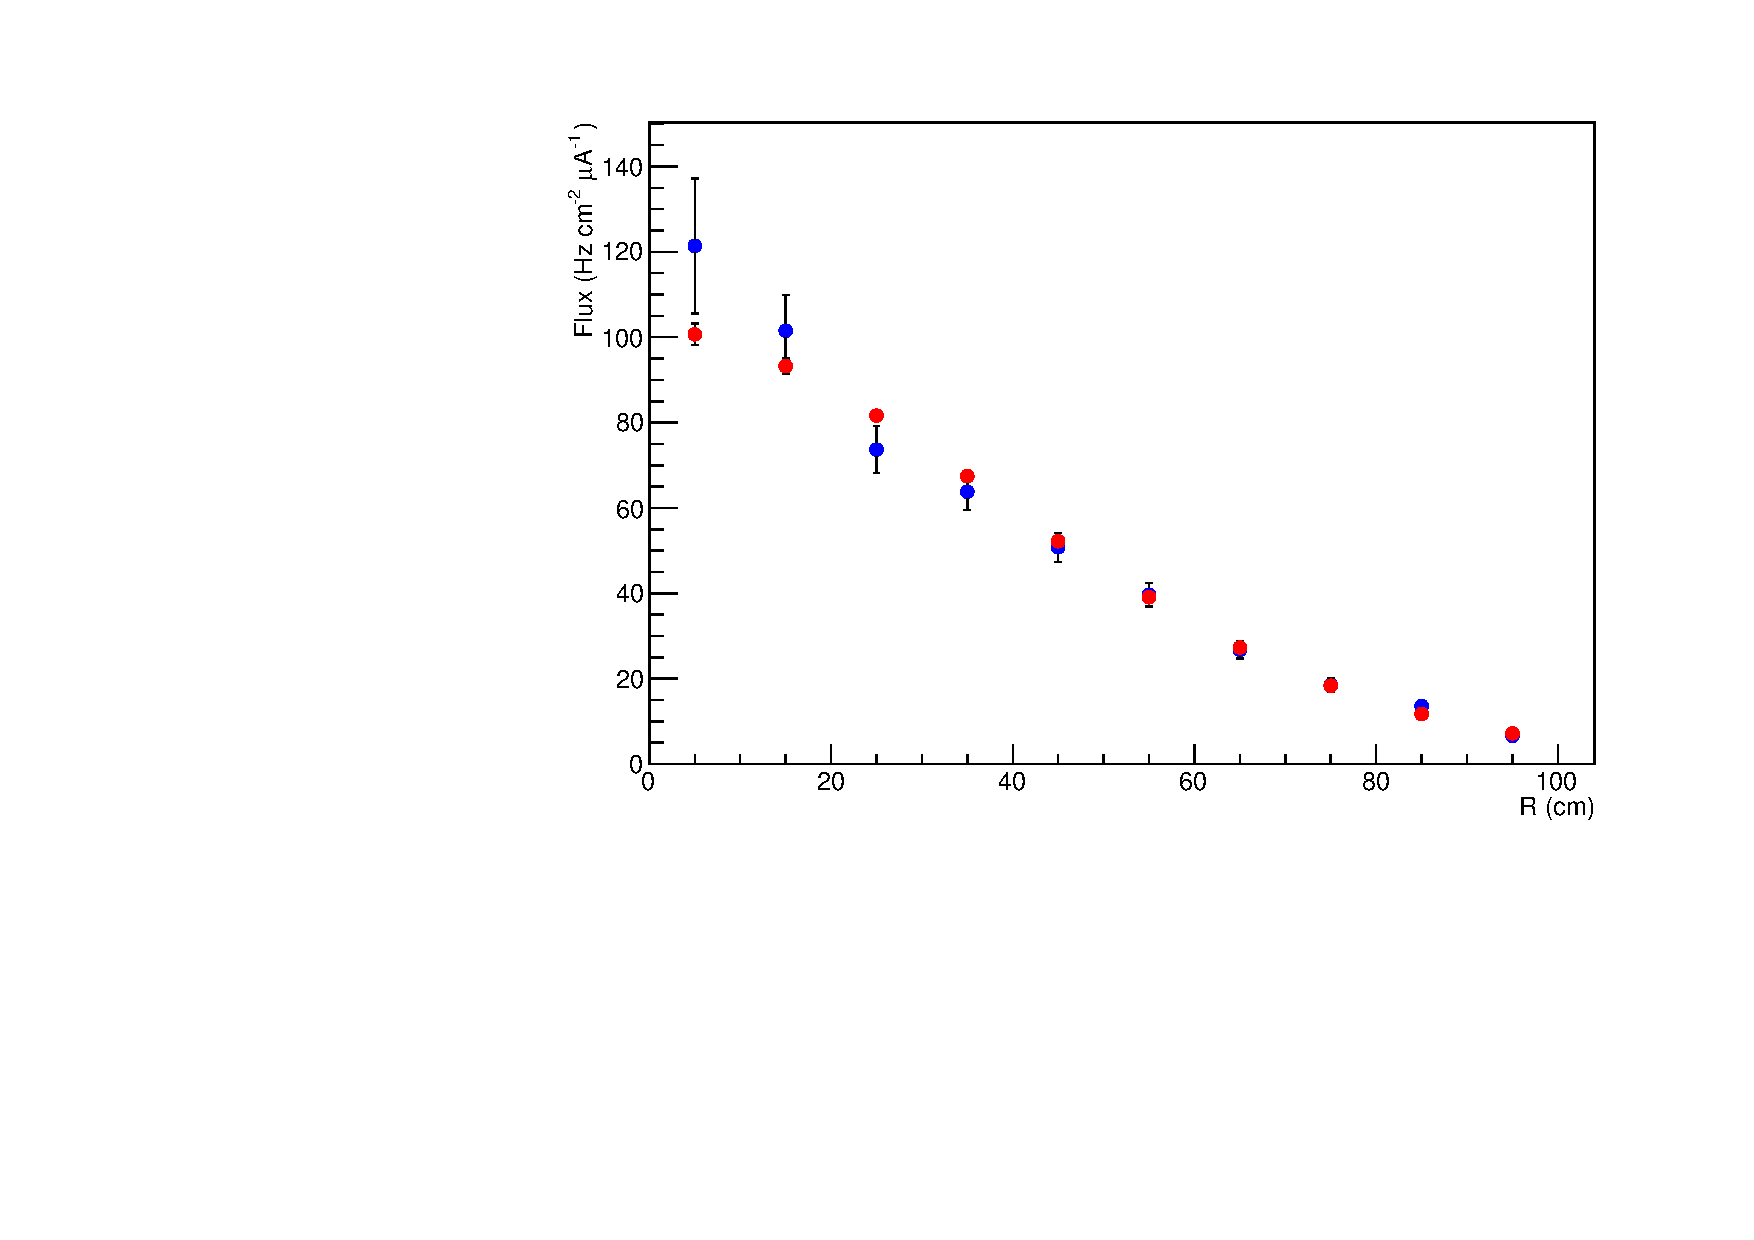
\includegraphics[width=7.7cm]{figs/SimVSGen.pdf}
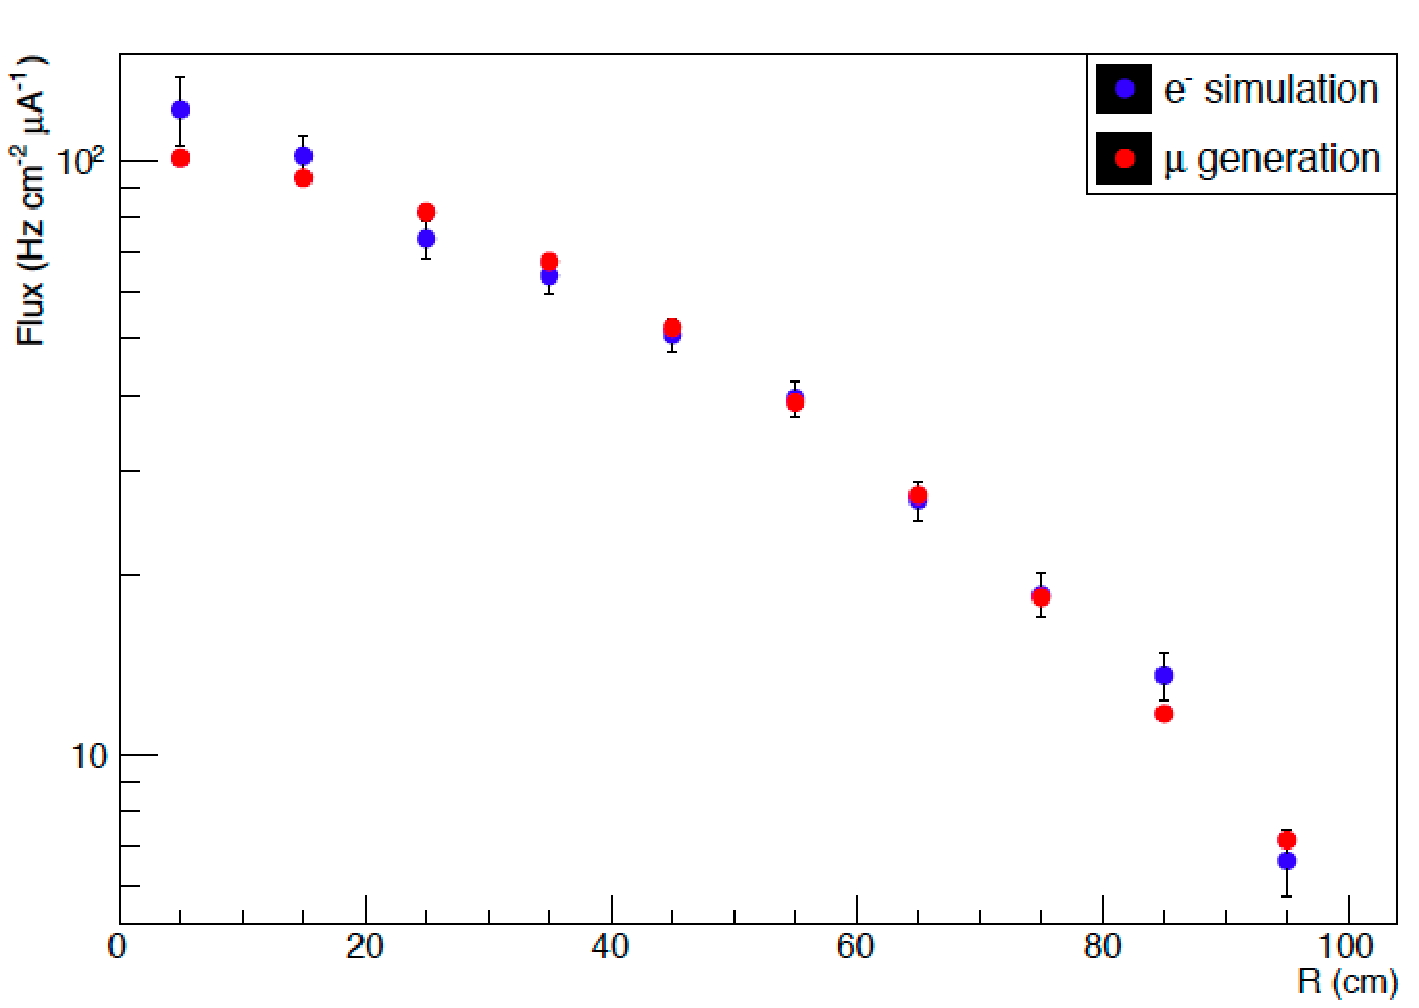
\includegraphics[width=7.0cm]{figs/mu-comp-far.pdf}
\caption{Muon kinetic energy vs. radial  distance from the beam-line axes obtained by GEMC (blue) and by the custom event-generator (red) at the sampling/ generation location (left) and in the region of interest (right) $\sim 20$ m downstream of the beam-dump.}
\label{fig:mu-sampling-extract} 
\end{figure}


\begin{figure}[h!] 
\center
\includegraphics[width=12cm]{figs/bg-csi.pdf}   
\caption{Energy deposited in the BDX-Hodo CsI(Tl) crystal by ALL crossing particles. The crystal has been located in the region of interest $\sim 20$ m downstream of the beam-dump. }
\label{fig:bg-csi}
\end{figure}

\subsubsection{Background - FLUKA}
We used FLUKA to estimate the background expected in the BDX-Hodo detector.
We simulated an 11 GeV electron-beam interacting with the beam-dump   and sampled the energy deposition in the BDX-Hodo CsI(Tl) crystal when located in the region of interest. 
Figure ~\ref{fig:bg-csi} shows the energy deposited in the crystal volume. The peak around XX MeV corresponds to MIPs crossing the crystal. The flux of MIPs derived  integrating the peak over a smooth background is in good agreement with the number of muons obtained by the full muon simulation with  GEMC. The remaining hits are mainly due to high energy neutrons interacting with the crystals and low energy neutrons captured by surrounding material. More details are reported in Sec.~\ref{sec:results}.
\begin{figure}[h!] 
\center
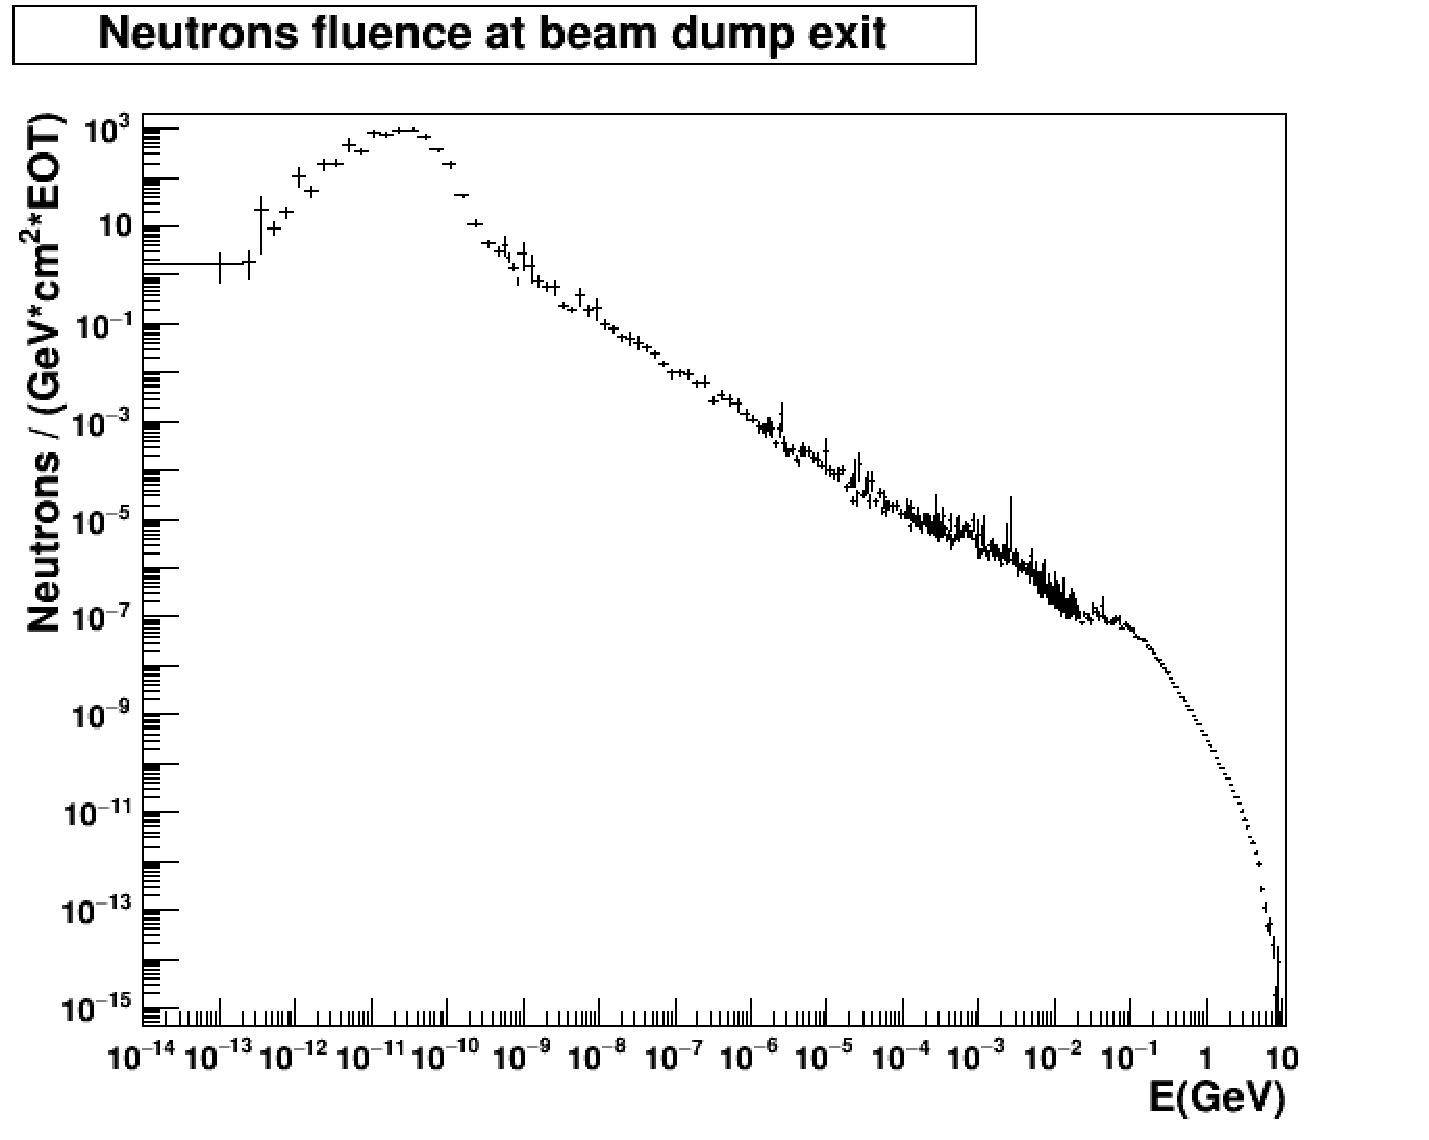
\includegraphics[width=7.5cm]{figs/NeutronsDump_1D.pdf}    
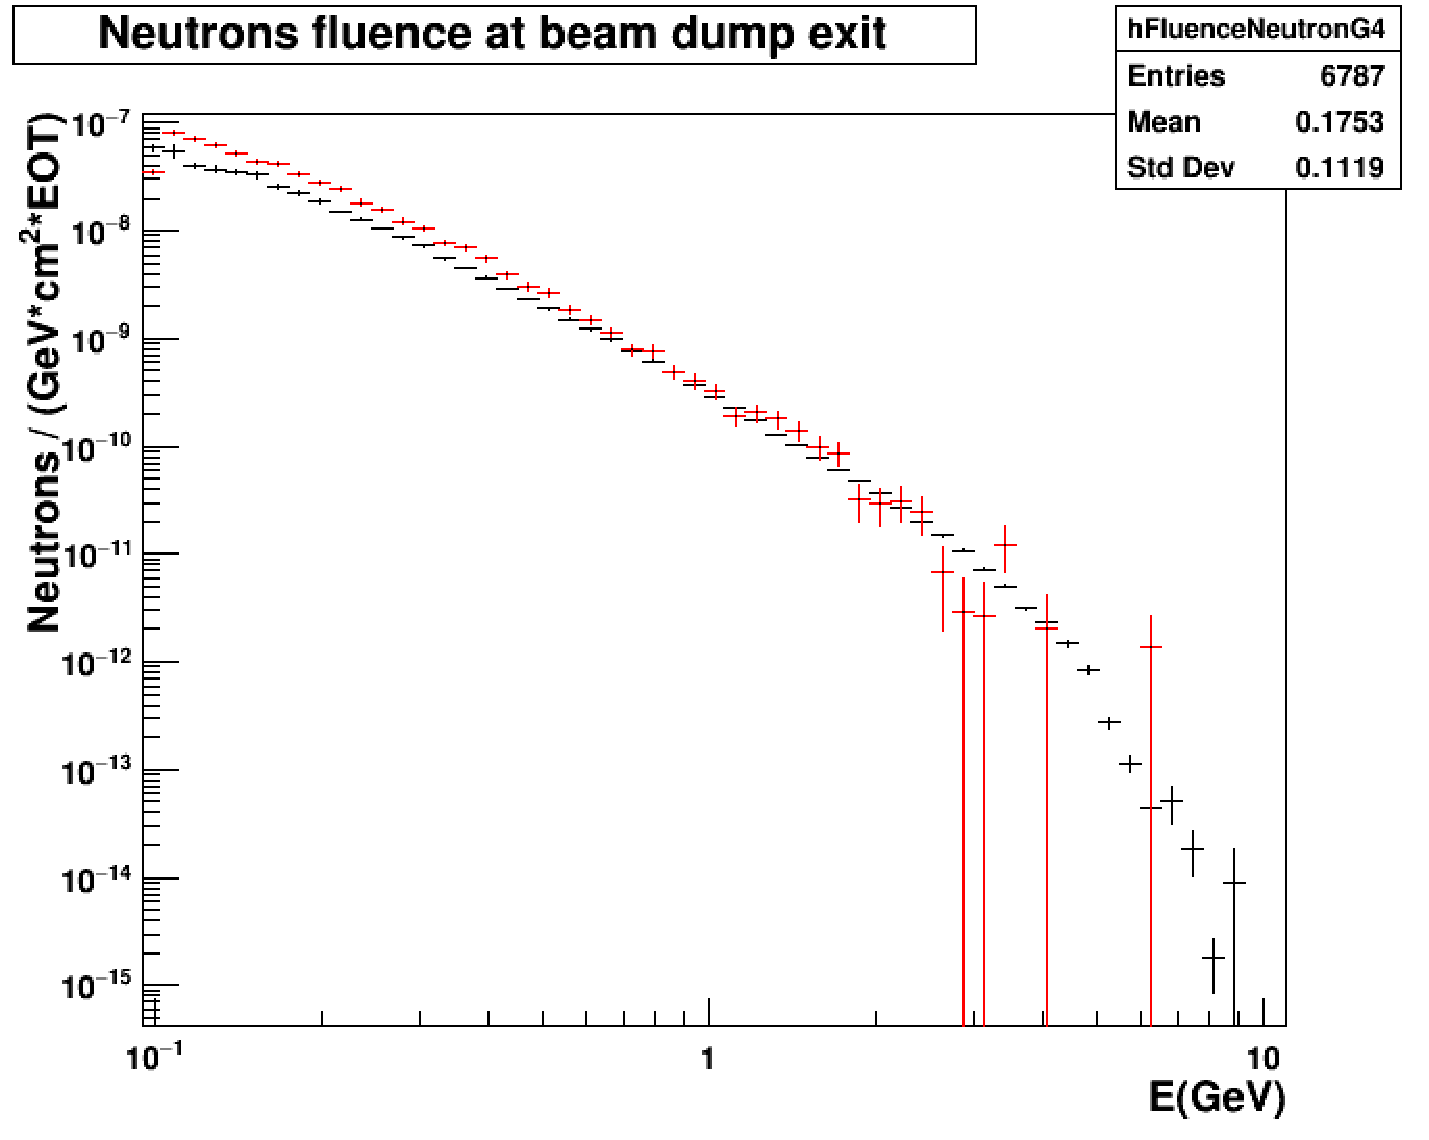
\includegraphics[width=7.5cm]{figs/NeutronsDumpComparison_1D.pdf}   
\caption{Neutron spectrum downstream of the the dump obtained by full FLUKA simulation (left). The right panel shows  the comparison between FLUKA (black) and GEMC (red) for the high energy part pf the spectrum.}
\label{fig:n-comp}
\end{figure}
It's interesting to note that the spectrum of  high energy neutrons , T$_n$> 100 MeV,  (sampled downstream of the dump)  obtained by GEMC is in good agreement with FLUKA (see Fig.~\ref{fig:n-comp}). The agreement indicates  that, in this energy range, both simulation tools are reliable. 

Another interesting aspect of the neutron spectrum is shown in Fig.~\ref{fig:n-lowE}. Here the energy spectrum (sampled downstream of the dump) obtained by FLUKA by RadCon (Ref.~\cite{jnote-bd}) is compared to the same plot obtained in our FLUKA simulations. The difference of the two runs is only in the different implementation of  beam-dump vault: a detailed description of the material surrounding the dump,  that includes air and concrete,  versus a simplified geometry/material description.   The effect is clearly visible in the low energy part of the spectrum (while the high energy part is almost identical) proving that a detailed description of the dump enclosure is necessary to correctly describe the produced backgrounds.
\begin{figure}[h!] 
\center
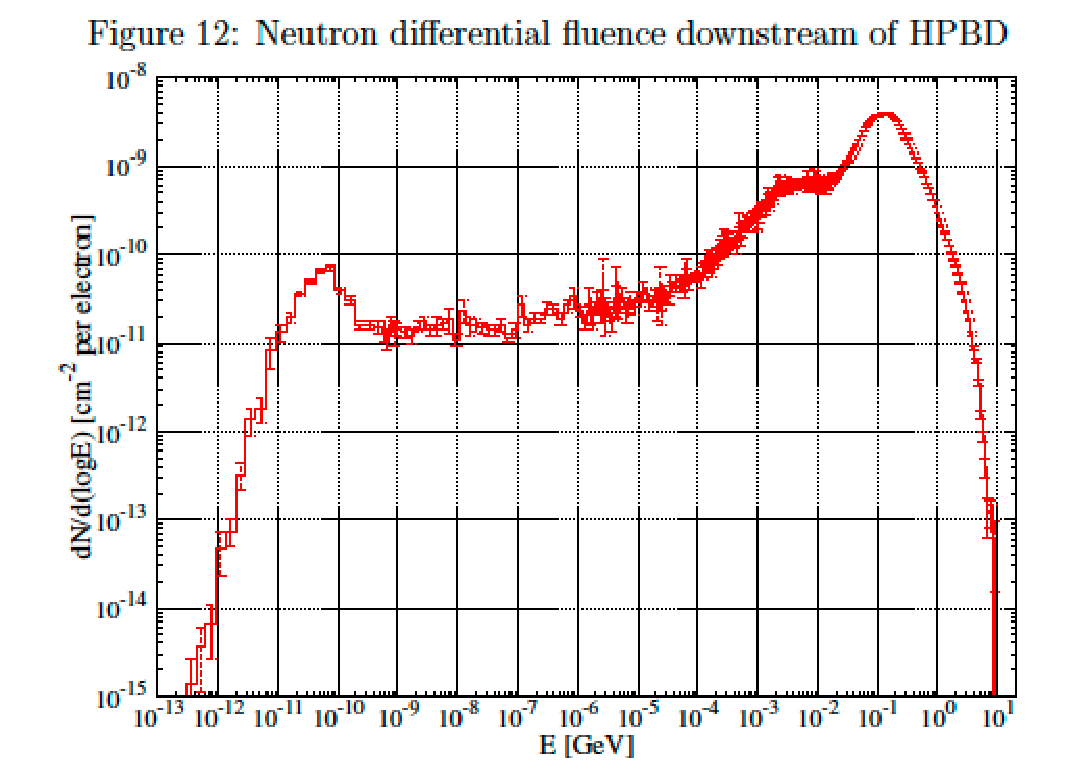
\includegraphics[width=7.5cm]{figs/bg-lowN-george.pdf}    
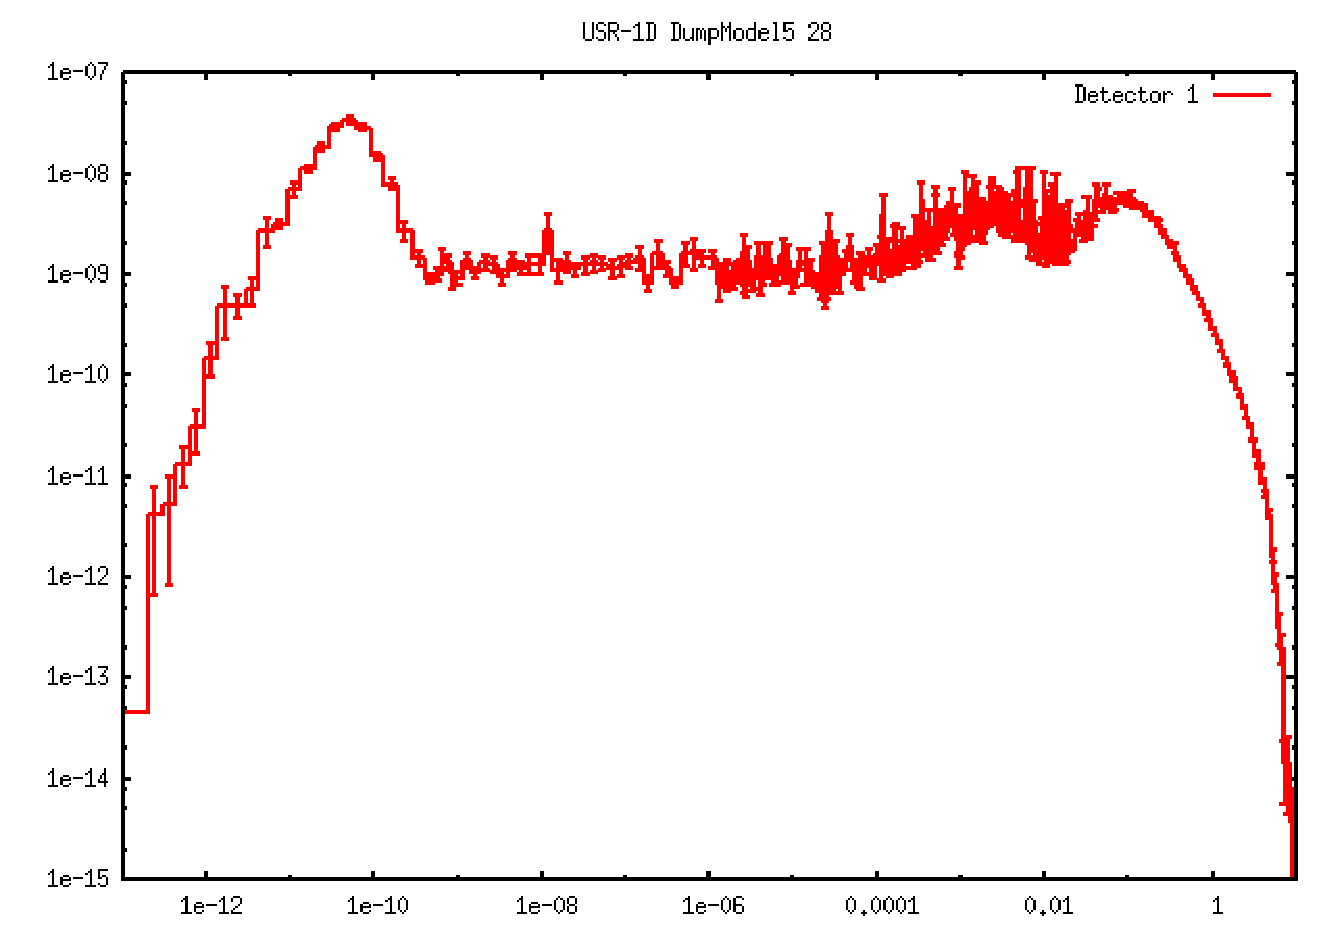
\includegraphics[width=7.5cm]{figs/NeutronsDumpComparisonDnDlogE_1D.pdf}   
\caption{Comparison of neutron energy spectrum obtained by FLUKA, sampled downstream of the beam-dump with a simplified geometry (left) and including vault sourrounding materials (right). The numeber of low energy neutrons significantly increases when the reflection on the wall is considered.}
\label{fig:bg-lowE}
\end{figure}
\\ \\ 
Muon and background flux  at  the location of interest will be discussed in details in the Sec.~\ref{sec:results} after presenting in the next Section,  the proposed experimental set up and the BDX-Hodo detector. 



